%File: feature.tex
%Date: Fri Jan 03 20:48:19 2014 +0800


\subsection{Feature Extraction}

\subsubsection{MFCC}
\label{sec:mfcc}
\textbf{Mel-Frequency Cepstral Coefficient} is a representation of the short-term power spectrum of a sound,
based on a linear cosine transform of a log power spectrum on a nonlinear mel-scale of frequency \cite{mfcc} .
MFCC is the mostly widely used features in Automatic Speech Recognition(ASR), and it can also be applied to Speaker Recognition task.


The process to extract MFCC feature is demonstrated in \figref{mfcc}
\begin{figure}

  \centering
  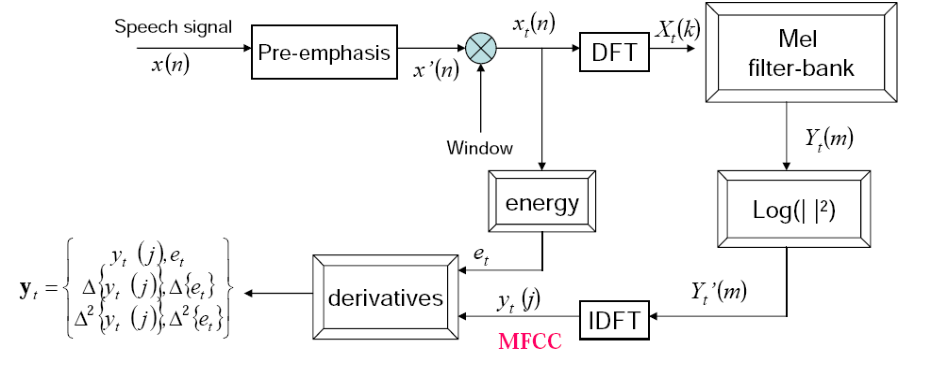
\includegraphics[width=\textwidth]{img/MFCC.png}
  \caption{MFCC feature extraction process\label{fig:mfcc}}

\end{figure}

First, the input speech should be divided into successive short-time frames of length $L$,
neighboring frames shall have overlap $R$.
Those frames are then windowed by Hamming Window, as shown in \figref{framming}.
\begin{figure}
  \centering
  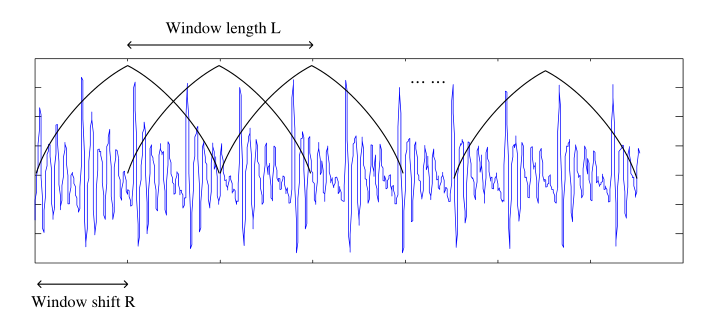
\includegraphics[width=0.7\textwidth]{img/MFCC-windowing-frames.png}
  \caption{Framing and Windowing \label{fig:framming}}
\end{figure}

Then, We perform Discrete Fourier Transform (DFT) on windowed signals to compute their spectrums.
For each of $N$ discrete frequency bands we get a complex number $X[k]$ representing
magnitude and phase of that frequency component in the original signal.

Considering the fact that human hearing is not equally sensitive to all frequency bands, and especially,
it has lower resolution at higher frequencies.
Scaling methods like Mel-scale are aimed at scaling the frequency domain to better fit human auditory perception.
They are approximately linear below 1 kHz and logarithmic above 1 kHz, as shown below in \figref{melscale}:
\begin{figure}[H]
  \centering
  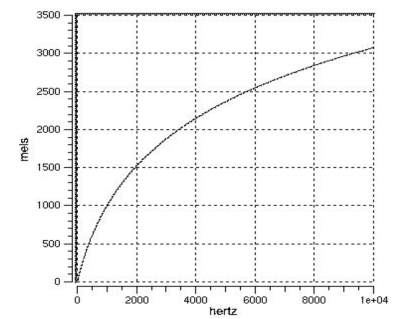
\includegraphics[width=0.5\textwidth]{img/mel-scale.png}
  \caption{Mel-scale plot \label{fig:melscale}}
\end{figure}

In MFCC, Mel-scale is applied on the spectrums of the signals.
The expression of Mel-scale warpping is as followed:
\[ M(f) = 2595 \log_{10}(1 + \dfrac{f}{700}) \]

\begin{figure}[H]
  \centering
  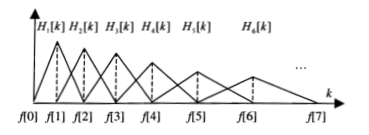
\includegraphics[width=0.5\textwidth]{img/bank.png}
  \caption{Filter Banks (6 filters) \label{fig:bank}}
\end{figure}
Then,  we appply the bank of filters according to Mel-scale on the spectrum,
calculate the logarithm of energy under each bank by $E_i[m] = \log (\sum_{k=0}^{N-1}{X_i[k]^2 H_m[k]}) $ and apply Discrete
Cosine Transform (DCT) on $E_i[m](m = 1, 2, \cdots M) $ to get an array $c_i $:
\[ c_i[n] = \sum_{m=0}^{M-1}{E_i[m]\cos(\dfrac{\pi n}{M}(m - \dfrac{1}{2}))} \]

Then, the first $k$ terms in $c_i $ can be used as features for future training.
The number of $k$ varies in different cases, we will further discuss the choice of $k$ in \secref{result}.

\subsubsection{LPC}
\textbf{Linear predictive coding} is a tool used mostly in audio signal processing and speech
processing for representing the spectral envelope of a
digital signal of speech in compressed form, using the information of a linear predictive model.\cite{lpc}

The basic assumption in LPC is that,
    in a short period, the $n$th signal is a linear combination of previous $p$ signals:
    $ \hat{x}(n) = \sum_{i=1}^pa_i x(n-i)$
    Therefore, to estimate the coefficients $ a_i$, we have to minimize the squared error
    $ \text{E}\left[ \hat{x}(n) - x(n)\right]$.
    This optimization can be done by Levinson-Durbin algorithm.\cite{levinson-durbin}

    Therefore, we first split the input signal into frames, as is done in MFCC feature extraction \secref{mfcc}.
    Then we calculate the $k$ order LPC coefficients for the signal in this frame.
    Since the coefficients is a compressed description for the original audio signal,
    the coefficients is also a good feature for speech/speaker recognition.
    The choice of $k$ will also be further discussed in \secref{result}.

